\chapter{METODOLOGIA}
\section{Abordagem da Pesquisa}
A pesquisa adotará uma abordagem X, conforme descrito por \citeauthor{ufpr2009} (\citeyear{ufpr2009}) em suas normas para elaboração de trabalhos acadêmicos. 

\section{Coleta de Dados}
Detalhamento dos procedimentos de coleta de dados.

\subsection{Figuras}
Qualquer que seja o tipo de Figura, sua identificação aparece na parte superior, precedida da palavra designativa (desenho, esquema, fluxograma, fotografia, gráfico, mapa, organograma, planta, quadro, retrato, imagem, entre outros), seguida de seu número de ordem de ocorrência no texto, em algarismos arábicos, travessão e do respectivo título. 

\begin{figure}[H]
    \centering
    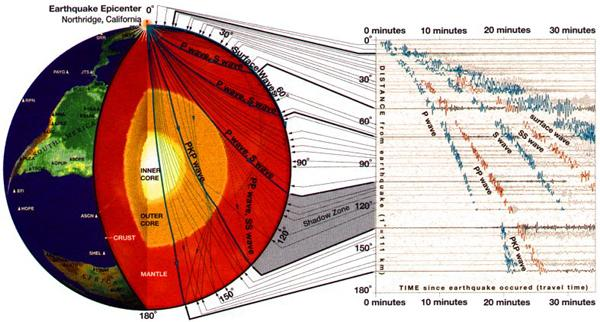
\includegraphics[width=0.8\textwidth]{figs/example-figure.png} % Placeholder for the image
    \caption{Limites operacionais de fator de potência para GDFV acima de 6kW. }
    \label{fig:limites_operacionais}
    \footnotesize
    Fonte: Adaptado de (ABNT, 2013). 
\end{figure}
Após a ilustração, na parte inferior, indicar a fonte consultada (elemento obrigatório, mesmo que seja produção do próprio autor), legenda, notas e outras informações necessárias a sua compreensão (se houver).  A Figura \ref{fig:limites_operacionais} deve ser citada no texto e inserida o mais próximo possível do trecho a que se refere. 

\subsection{Tabelas}
Nesta seção será feita a demonstração do uso de tabelas no trabalho acadêmico.  Uma tabela deve apresentar dados numéricos de modo resumido e é utilizada principalmente para a apresentação de comparações. 

\begin{table}[H]
    \centering
    \caption{Instituições de Educação Superior (IES) por Organização Acadêmica. }
    \label{tab:ies_org}
    \begin{tabular}{lcc}
        \toprule
        \textbf{Organização Acadêmica} & \textbf{IES} & \textbf{\%} \\
        \midrule
        Universidades & 169 & 8,4 \\
        Centros Universitários & 107 & 5,3 \\
        Faculdades Integradas & 119 & 5,9 \\
        Faculdades, Escolas e Institutos & 1474 & 73,2 \\
        Centros de Educação Tecnológica e Faculdades de Tecnologia & 144 & 7,2 \\
        \midrule
        \textbf{Total} & \textbf{2013} & \textbf{100} \\
        \bottomrule
    \end{tabular}
    \footnotesize
    Fonte: Censo da Educação Superior 2004 (INEP, 2004). 
\end{table}
Deve-se seguir tal padrão em todo o trabalho, constando também na lista de tabelas, separada da lista de ilustrações.  Os quadros não devem ser chamados de tabelas, uma vez que se diferenciam destas por apresentarem as laterais fechadas e o conteúdo não numérico.  As tabelas que ocupem mais de uma folha devem ter continuidade na folha seguinte, repetindo o título e o cabeçalho da tabela e colocando-se uma linha horizontal de fechamento apenas no final da tabela.  Segue um exemplo a seguir na Tabela \ref{tab:ies_org}. 

\subsection{Equações}
Para facilitar a leitura das equações, a fim de que comporte seus elementos (expoente, índices e outros), sugere-se a separação por uma linha com espaçamento 1,5 das equações e fórmulas. 

$$ x=\frac{-b\pm\sqrt{b^2-4ac}}{2a} \quad (1) $$

Ao longo do texto, quando o mesmo contiver diversas fórmulas e equações, estas devem ser identificadas com números sequenciais, colocados entre parênteses, na extremidade direita da linha, junto à margem. 

$$ (x+a)^n=\sum_{k=0}^n \binom{n}{k}x^k a^{n-k} \quad (2) $$
